\documentclass{article}

% Language setting
% Replace `english' with e.g. `spanish' to change the document language
\usepackage[english]{babel}
\usepackage{amsfonts}
% Set page size and margins
% Replace `letterpaper' with`a4paper' for UK/EU standard size
\usepackage[letterpaper,top=2cm,bottom=2cm,left=3cm,right=3cm,marginparwidth=1.75cm]{geometry}

% Useful packages
\usepackage{amsmath}
\usepackage{graphicx}
\usepackage[colorlinks=true, allcolors=blue]{hyperref}


\begin{document}


\section{Info on noise on Pulser device}

Pulser device is Chadoq. This table sums the main characteristics of noise parameters

\begin{figure}[h!]
	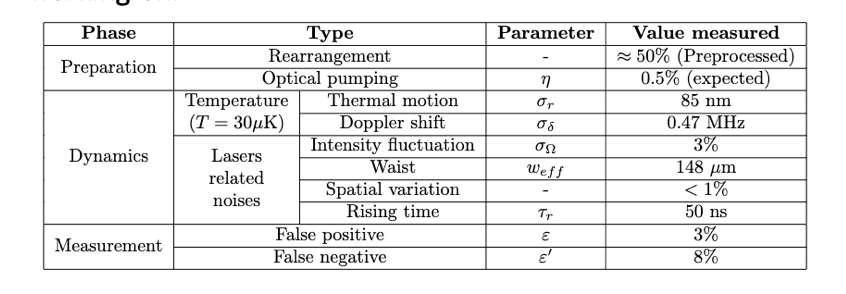
\includegraphics{info_q}
\end{figure}

From Lucas' email:

\begin{itemize}
	\item For the optimisation, your pulses should not be shorter than approximatively twice the rising time. The fact that the pulses are not perfect square induces a small change in the overall phase applied. 
Also the total sequence should not last longer than 5 us because after that the decoherence effects become strong enough and should be taken into account.

	\item For the interaction term, we are working with a certain rydberg level at the moment which can be defined in Pulser by n = 60 (this should return an interaction coefficient of $2 \pi \times 137 000$ $MHz \mu m^6$). You can change that at the beginning of your code when importing from the Device class the instance Chadoq2 and then do Chadoq2 change rydberg level(60).
	
	\item For the new design of the sequence, it depends a bit on how you parameterize your QAOA. For instance for odd intervals of time, you apply $\frac{\Omega_{on}}{2 \pi} = 2 MHz$  and no detuning. For even intervals, you apply $\frac{\Omega_{on}}{2 \pi} = 0 MHz$ (no amplitude) but then you need to apply (in order to mimic the prototype implementation) $\delta = lightshift(\Omega_{on}) - lightshift(\Omega_{off})$ which should be around $2 \pi \times -3 MHz$. 
The function lightshift is given by 

\begin{align}
	lightshift(\Omega) = \frac{\Omega_r^2-\Omega_{\text{b from } \Omega}^2(\Omega)}{4 \Delta_i} \\
	\Omega_{\text{b from } \Omega}(\Omega) = \Omega \frac{2 \Delta_i}{\Omega_r}
\end{align}

with $\Delta_i = 2\pi \times 700$ and $\Omega_r = 2 \pi \times 30$.

So taking $\Omega_{on} = 2 \times 2 \pi $ MHz and $\Omega_{off} = 0 \times 2 \pi $ we get:

\begin{align}
	\delta &= lightshift(\Omega_{on}) - lightshift(\Omega_{off}) \\
	 &= \frac{\Omega_r^2 - (2\times 2\pi \frac{2 \Delta_i}{\Omega_r})^2}{4 \Delta_i} - \frac{\Omega_r^2}{4 \Delta_i} \\
	 &= -\frac{(2\pi)^2 (4 \frac{2\pi \times 700}{2 \pi \times 30})^2}{2 \pi \times 4 \times 700} = -(2 \pi) \frac{280}{90} = -3.1 \times 2\pi
\end{align}
\end{itemize}

\end{document}